\chapter{Implantation detector development} \label{ch:yso_detector}

\section{Particle Detection using Scintillators}
Scintillators are one of the oldest materials to be used for particle detection and identification. The idea of using the scintillators dates back to the early 1900s \citep{rutherford} when Ernest Rutherford discovered $\alpha$-particles with the aid of scintillator Zinc sulfide (ZnS). In the following years huge strides were made in the development and implementation of these materials in various sectors of research and industry.\\

The materials falling under the category of scintillators are broadly categorized as organic and inorganic scintillators. The scintillation mechanism depends on the structure of the crystal lattice. Here the focus is on inorganic scintillators (halides, oxides, chalcogenides, and glasses). The basic concept behind the particle or incident gamma-ray detection using a scintillator is the conversion of the energy lost in the material into light, which is emitted in a specific wavelength band of the Electromagnetic spectrum. 
The ionizing radiation upon interaction leaves the system in a state of non-equilibrium, and the tendency to reach a state of equilibrium is lead by a multitude of elementary processes, such as the creation of primary electronic excitation which will produce an avalanche of secondary particles including electrons, holes, photons, and plasmons. These electronic excitations produce numerous thermalized electron-hole(e-h) pairs and low energy excitons which ultimately transform into light photons, i.e., scintillation. The following steps can broadly describe the scintillation process:
\begin{enumerate}
	\item Absorption of the ionizing radiation and creation of primary electrons and holes.
	\item Relaxation of the primary electrons and holes, thereby production of many secondary electrons, holes, protons, plasmons, and other electronic excitations.
	\item Thermalization of the low-energy secondary electrons (holes) resulting in a number if e-h pairs with energy roughly equal to the band-gap energy $E_{g}$.
	\item Energy transfer from e-h pairs to the luminescence centers and their excitation.
	\item Emission from the luminescence centers.
\end{enumerate}
\begin{figure}[h!]
	\centering
	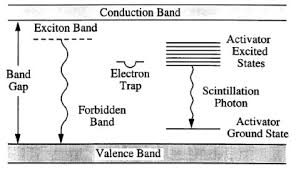
\includegraphics[width=10cm,height=8cm]{figures/inorganic_scintillators_mechanism.jpeg}
	\caption[A schematic diagram explaining the scintillation]{A schematic diagram explaining the scintillation mechanism in inorganic scintillators. }
	\label{fig:scintillation_mechanism}
\end{figure}



\subsection{Charged Particles}
A charged particle in its passage through the volume of the material exhausts its kinetic energy in excitation and ionization of atoms. These kinds of energy losses are labeled as ionization losses. What we observe then is a statistical average of the two processes occurring as the particle slows down. The stopping power S (dE/dx) of the matter is determined concerning the energy lost (dE) by the particle in infinitesimal distance (dx): the higher the stopping power, the shorter the range into the material the particle can penetrate. The quantity S is also referred to as \textit{specific energy loss}. The average ionization losses of a charged particle are given by the well known Bethe-Bloch formula \citep{bethebloch}.

\begin{equation}
-\frac{dE_{ion}}{dx}=\frac{4\pi N_{A} Z^{2} e^{4}}{m_{e} V^{2}} \frac{z}{a} \Bigg[ ln\Bigg(   \frac{2mV^{2}}{\overline{I} (1-\beta^{2})}    \Bigg) -\beta^{2}\Bigg],
\end{equation}


Where z, m, and V are the charge, mass, and velocity of the particle, respectively; \textit{x} (cm\textsuperscript{2}/g) is the path of the particle into the matter; Z and A are the atomic and mass number of the matter, respectively; $N_{A}$ is the Avogadro number, and $\overline{I}$ is usually obtained empirically, but some estimates are made using the relation $\overline{I}$ = 13.5 Z (ev).
\newline
Following above equation, it can be inferred that ionization power of heavy charged particle (proton, $\alpha$ particle, multiply ionized atoms, etc.) is $z^{2}$ times greater than the ionization power of an electron of the same velocity. Low-energy electrons, protons, $\alpha$ particles, and heavy ions are weakly-penetrating particles requiring small scintillator thickness for stopping. The light output of the scintillator depends not only on the energy losses but also on the density of ionization. In spite of ionization losses increasing with increase the charge  and mass of the particle, there is a decline in the light output of the scintillator.

The light produced in the scintillating material by highly ionizing particles (heavy ions) is lower than that produced by electrons of the same energy. Therefore, the signal generated by the ions will be seen at lower voltages than their real values for a scintillator calibrated with electrons or $\gamma$-rays, due to the presence of light-quenching for heavy ions. A knowledge of these transformation factors is very important when it comes to detecting and interpreting heavy ions. 
Light yield dL is proportional to the energy-loss (dE) by the particle in the scintillator
\begin{equation}
dL = SdE
\end{equation}

where S is the absolute scintillation factor. In differential form, the above equation is written:

\begin{equation}
\frac{dL}{dx}= S\frac{dE}{dx}
\end{equation}

The suppression for the light yield for the heavy ions is suggested by Birks Relation

\begin{equation}
\frac{dL}{dx}= S\frac{\frac{dE}{dx}}{1+kB\frac{dE}{dr}}
\end{equation}

where B$\frac{dE}{dx}$ denotes the density of excitation centers along the track, k is the quenching factor; kB as a product is known as Birks Factor. The quenching factor for ions is the ratio of the light yield of ions relative to that of electrons at the same energy.

\begin{equation}
Q_{i}(E)=\frac{L_{i}(E)}{L_{e}(E)}
\end{equation}


\*Explain Quenching from physics point of view*\ Look in the birks book 


\subsection{Neutrons}
Neutrons interact with a solid mainly through strong interplay with the nuclei. The interaction of neutrons with the matter is mainly restricted to scattering and absorption. Elastic scattering cross-section of neutrons at low energy is given as:
\begin{equation}
\sigma_{n}=4\pi(1.4 \cdot 10^{-13} A^{1/3})^{2}
\end{equation}
Usually, crystals based on B-, Li-, and Cd are used as scintillators for detecting low energy neutrons because of the large cross-section of the elements for neutrons. With increasing energy of neutron, inelastic scattering starts to dominates.

\section{YSO (Yttrium Ortho Silicate) based Implant Detector}

Implantation detectors are employed at fragmentation beam facilities mainly to detect the tagged isotopic beam impinged on it. The impinged ions, by eventually coming to rest in the scintillator, undergo radioactive decay emitting low energy beta particles, $\gamma$-rays, alpha particles, and neutrons. Thus, a proper mechanism is needed to identify the impinged ions and correlate them to the corresponding beta event. The correlations are crucial for determining the decay half-lives, and developing decay cascade of the precursor nuclei into subsequent daughter nuclei. The correlations are drawn on a position-to-position basis of the impinged ions and the beta particles. The detector is also needed to properly tag the gamma, neutron, or alpha events for exploring the full decay perspectives of nuclei: it is helpful in calculating the branching ratios, half-lives, and energy for various decay chains- the energy of particles to be detected range from a few keV to GeV. At present, most facilities around the world, are using detectors which are silicon-based, such as AIDA \citep{AIDA}, and WAS3ABi \citep{wasabi} at RIBF, RIKEN. These detectors work well overall but fail to posses good timing resolution needed for measurements bases on Time of Flight (ToF). Further, YSO has higher stopping power than Si, requiring lesser material thickness for stopping energetic ions and also provides high light yield.
In the following section details about the construction and performance of the detector are presented.




/*Put the Rationale behind the selection of the material YSO

Discuss about its characteristics in terms of the timing and the fact that it can be segmented,
put the characteristics table here in the section.*/


YSO ($Y_{2}SiO_{5}$:Ce) scintillation crystal ($\rho$=4.44 \textit{g/$cm^{3}$}, effective Z=39) offers a good combination of properties characterizing an implantion detector. YSO emission spectrum peaks at 420 nm (refractive index = 1.8) and couples well with PSPMT under the stimulation of high energy. It also has the advantage of high light yield, good timing-resolution, short decay time, non-deliquescence, and all-around stable physical and chemical properties \citep{ysospecs}.

Using YSO, a new segmented scintillator-based detector was developed at the University of Tennessee, Knoxville. The detector unit consists of a segmented (2inch x 2inch) YSO crystal with each segment having a dimension of 1 mm $\times$ 1 mm. Each segment, as well as the face and the sides, is isolated by ESR (3M) reflector material. The crystal has a thickness of 5mm and is coupled with a flat panel multi-anode position-sensitive photo-multiplier (PSPMT) tube by Hamamatsu, H12700. There is a 2-mm thick quartz light diffuser between the YSO crystal and the PSPMT to achieve sub-anode position resolution by spreading the light from one pixel onto several anodes of the PSMT. The crystal is coupled with PSPMT using organic adhesive material, sylgard, to provide mechanical rigidity to the final detector. This design was used for BRIKEN Fall 2017 campaign.

The signals from the PSPMT are read out using a resistor network board provided by Vertilon. Signals from the detector are decoded into a position array by calculating the \textit{centroid} of the signal voltage, using what is known as \textit{Anger Logic}, also named after Hal Anger \citep{angerlogic}, who implemented it to get the positions of the nuclear events in $\gamma$-ray detectors. The idea behind Anger Logic is conceptualized as follows: if the voltage signal of a photomultiplier is made proportional to its position, the \textquotedblleft  centroid\textquotedblright of the voltages produced by a particle will determine where the particle originated-the goal of this logic. Anger Logic is needed to enhance spatial resolution; large thicknesses of scintillator material are required to improve the photon cross-section and the measurement of the photon energy, which is essential for suppression of the contribution from Compton-scattered photons. Furthermore, the segmentation of the scintillator supplements the position resolution of the particle hit-pattern. 

\subsection{YSO Detector Development for ToF based Delayed Neutron Spectroscopy}
A YSO implant detector with revised design and specifications was developed for performing ToF-based delayed neutron emission spectroscopy using VANDLE \citep{VANDLE}. The detector acts as a fast $\beta$-trigger along with recording implanted ion positions.

\subsubsection{Detector design and construction}
The detector consists of a 7.5 cm $\times$ 7.5 cm segmented array of YSO crystal with 2 mm pitch, coupled with a PSPMT by Hamamatsu, H12700B-03 (48.5 mm $\times$ 48.5 mm effective area), via a tapered and pixelated acrylic light guide. The light guide is used to focus the light produced through scintillation in YSO onto the face of the PSPMT. A one-to-one correspondence between the pixels of the crystal and the light guide is ensured by UV curing the two with each other. The combined crystal and light guide system is coupled with the PSPMT using sylgard, providing optical coupling and mechanical stability. 
\begin{figure}[h!]
	\centering
	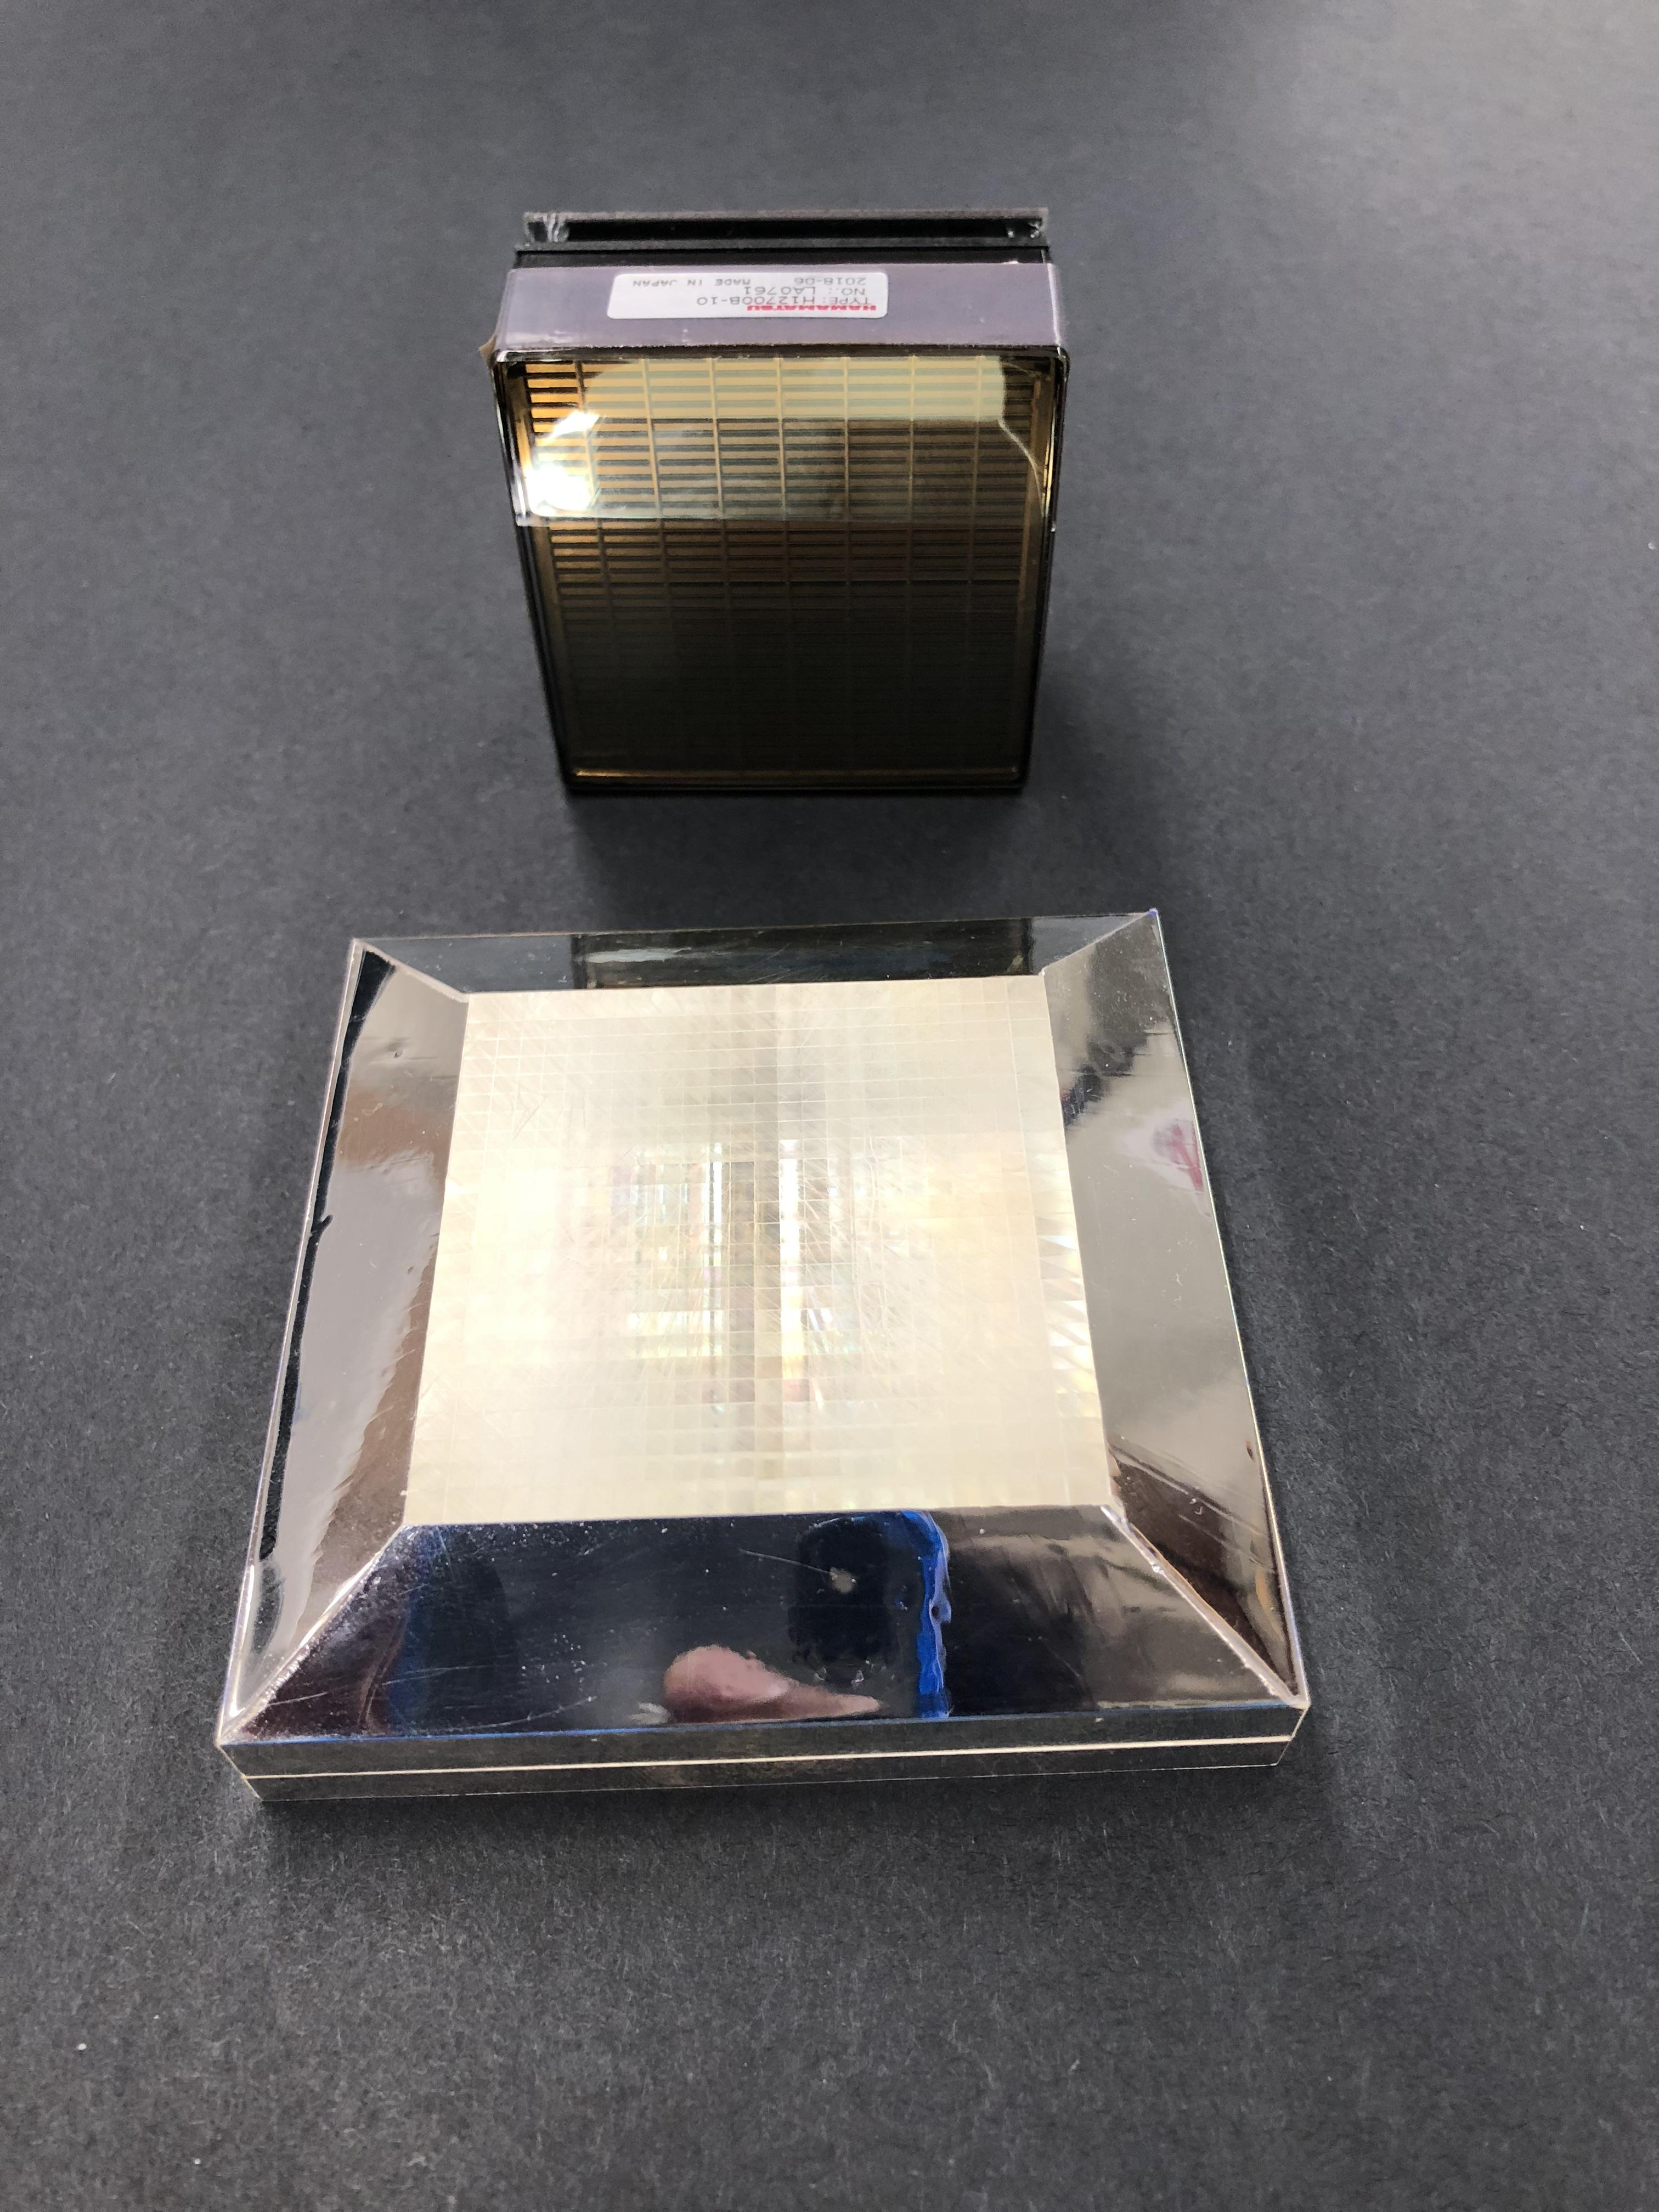
\includegraphics[width=7cm,height=7cm]{figures/new_yso_tapered_light_guide.jpg}
	\caption[The image above shows the crystal and light guide]{The image above shows the crystal and light guide combination, and the PSPMT used. The sides of the light guide are covered with ESR to ensure no light escaping.}
	\label{fig:yso_light_guidel}
\end{figure}
The sides of the connection are sealed with epoxy glue to ensure stronger support. This variant of the implantation detector has a larger area to capture a more divergent beam spot. \\
ToF is defined as follows:
\begin{equation}
\textit{ToF}=T\textsubscript{n}-T\textsubscript{$\beta$}
\end{equation}
where $T\textsubscript{n}$ is the time stamp of the neutron events recorded in VANDLE, and $T\textsubscript{$\beta$}$ is the time stamp of the beta events triggering YSO.

The energy of the neutrons can be deduced by the relation as follows:

\begin{equation}
E=\frac{1}{2} \times m_{n} \times  \frac{ L^2}{ ToF^{2}}
\end{equation}
where m\textsubscript{n} is the neutron mass, ToF is the Time of Flight, and L is the flight path. 

\begin{equation}
\frac{\Delta E}{E}  = \sqrt{\Bigg[\frac{2\Delta L}{L}\Bigg]^2 + \Bigg[\frac{2\Delta t}{t}\Bigg]^2}
\end{equation}

Where $\Delta L$ has contributions from the uncertainty in position measurement of electrons in YSO, and neutrons in VANDLE \citep{VANDLE}, $\Delta t$ is the timing-jitter, which is given by the root mean square of the timing resolution of YSO and VANDLE. $\Delta t$ in total encapsulates contributions from jitter induced by transit-time variance of photons in scintillator,  PSPMT response, digital electronics, and intermediate noise. 

\begin{figure}[h!]
	\centering
	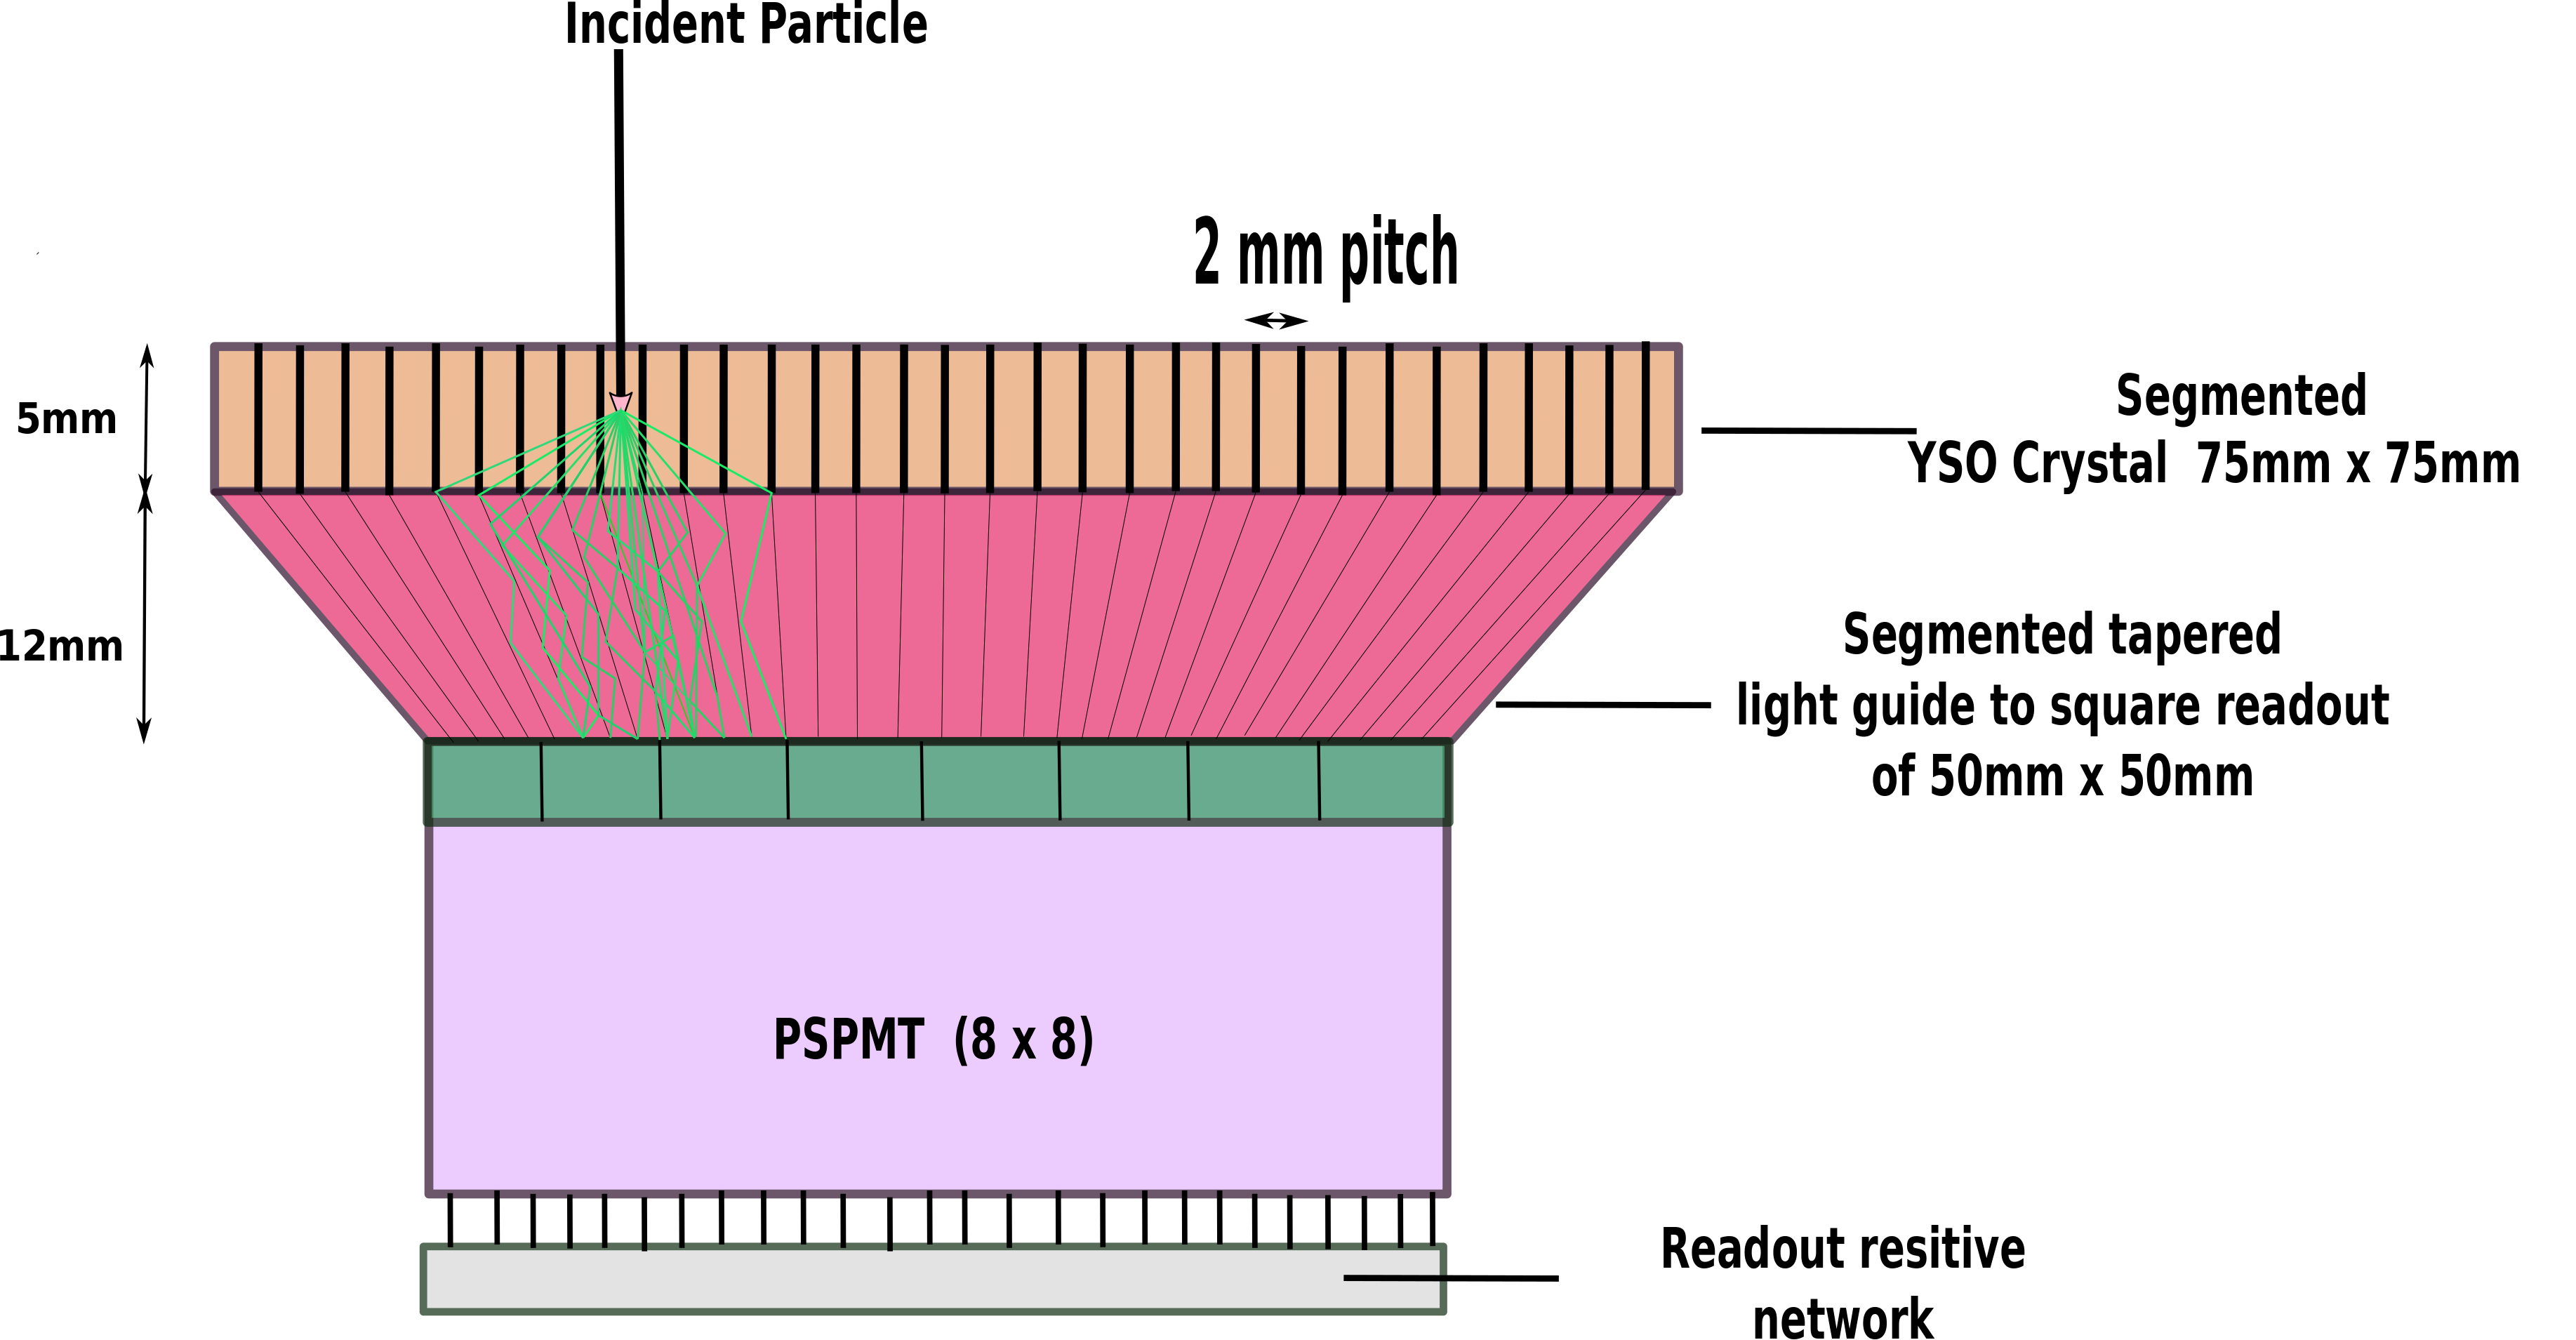
\includegraphics[width=14cm,height=8cm]{figures/yso_lightguide.png}
	\caption[A graphical depiction of the detector design]{A graphical depiction of the detector design, showing the placement of YSO crystal and light guide on PSPMT. Pathway of photons on its way to the sensor is through the light-guide.}
	\label{fig:yso_riken_2018}
\end{figure}
\newpage
\begin{figure}[h!]
	\centering
	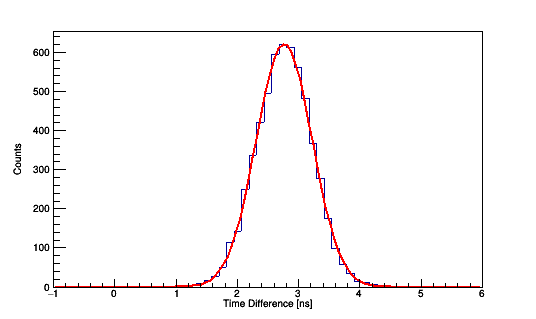
\includegraphics[width=12cm, height=8cm]{figures/YSO_timing.png}
	\caption[Time difference between the signals having gates]{Time difference between the signals having gates for energy above the Compton edge of \textsuperscript{60}Co. This configuration offers a timing resolution of $\sim$ 650 ps at 600 V. }
	\label{fig:time_resolution}
\end{figure}

From the above relation, uncertainty in the energy arise from the position and timing precision in both YSO and VANDLE. The position uncertainty for betas in YSO is of the order of mm, on the other, hand position uncertainty for neutrons is of the order of cm in VANDLE. Thus, VANDLE position uncertainty dominates in determining energy uncertainty. Timing resolution has equal contributions from both the detectors. A few tests were done to deduce the timing resolution of the YSO detector for signals representing various energy ranges. 

\begin{figure}[h!]
	\centering
	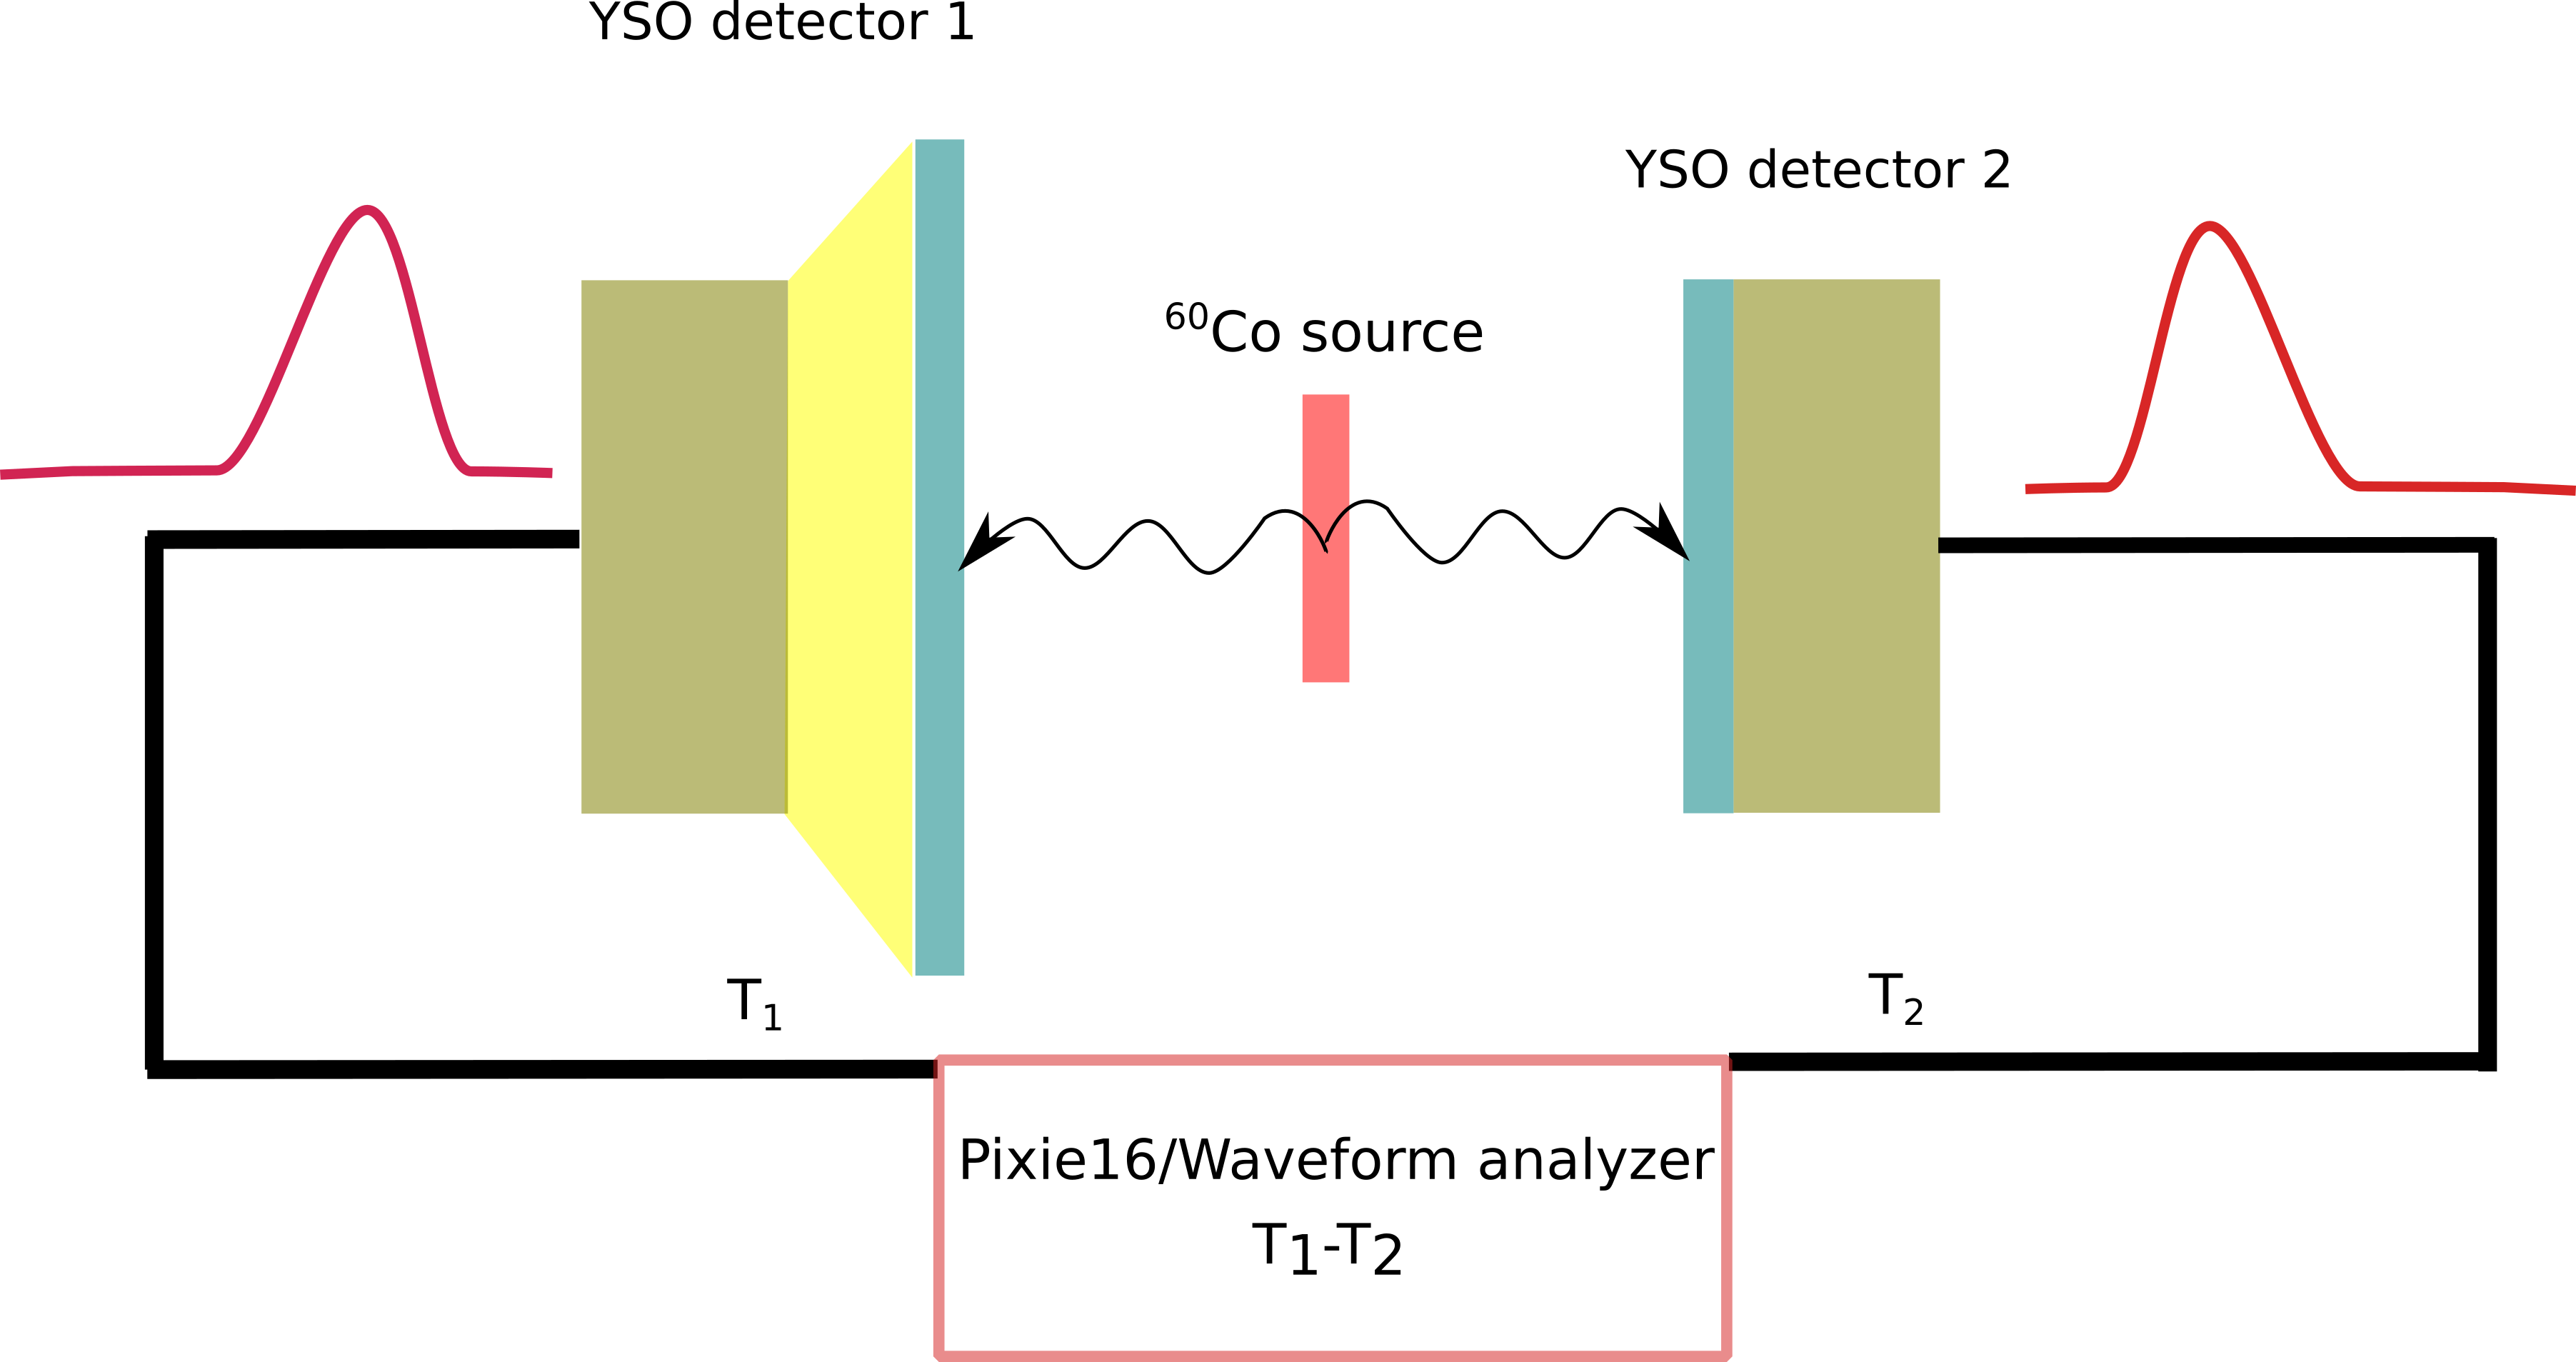
\includegraphics[width=16cm, height=10cm]{figures/yso_timing_test.png}
	\caption[]{Schematic of the setup for YSO timing measurement. }
	\label{fig:timing_measurement}
\end{figure}


The tests were done to ensure a good timing resolution for the actual experimental run. The criteria involved getting the time stamp of the same event in two similar YSO detectors using a \textsuperscript{60}Co source, and plotting the distribution of the difference in time, recorded in the two detectors. The distribution can be approximated to be Gaussian in nature. The Full-Width Half-Maximum (FWHM) of the distribution gives an estimate of the timing-resolution of both the detectors combined. Single detector resolution can be deduced assuming an equal uncertainty contribution for both the detectors. Scenarios with different biasing voltage were also explored. The detector, on average, has a timing resolution better than $\sim$ 600 ps for signals representing energy $\geq$ 1 MeV. Several other tests were performed to check the image quality, quality of coupling, and position resolution. 

\begin{figure}[h!]
	\centering
	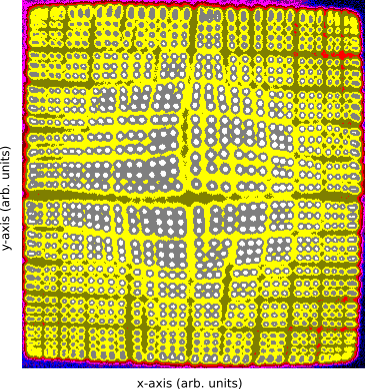
\includegraphics[width=9cm,height=9cm]{figures/yso_inkscape1.png}
	\caption[Flat-field image produced using \textsuperscript{137}Cs source on]{Flat-field image produced using \textsuperscript{137}Cs source on \textit{x-y} plane (arbitrary scaling) showing each pixel well-illuminated. The crystal is 7 cm $\times$ 7 cm with each pixel having dimension 2mm $\times$ 2mm. The gaps are present in the image because of the light guide being constructed out of four different sections and joined together. The pixels on the corner are more crowded because of the relatively more tapering of the light guide along the z-axis for the edges than for the center.}
	\label{fig:flood_field_image}
\end{figure}
\subsubsection{Range Distribution of Ions and Electrons in YSO}


/*Insert the test images gain for example for Sr90 and Cs137*/
/*Also insert the individual signals*/
/**/

Exotic isotopes present in the cocktail beam are highly energetic having the energy of the order of GeV. An estimate of the range of these ions in YSO crystal is important from the point of view of the experiment, where collecting ample statistics is of prime concern. These estimates are also important for detector design, helpful in choosing the right thickness of the scintillating material. \textbf{LISE++} \citep{lise} is a software that has been developed to calculate the transmission and yields of fragments produced and collected in a spectrometer. The LISE++ code may be applied at medium-energy and high-energy facilities (fragment- and recoil-separators with electrostatic and magnetic selections). In a number of facilities, like A1900 and S800 at NSCL, LISE3, SISSI/LISE3, and SPEG at GANIL, FRS and SuperFRS at GSI,  RIPS and BigRIPS at RIKEN, based on the separation of projectile-like and fission fragments,  fusion residues are included or might be easily added to the existing optical configuration files. The range estimates of ions produced can be deduced for any material by providing chemical properties of the material to LISE.
\newpage
\begin{figure}[h]
	\centering
	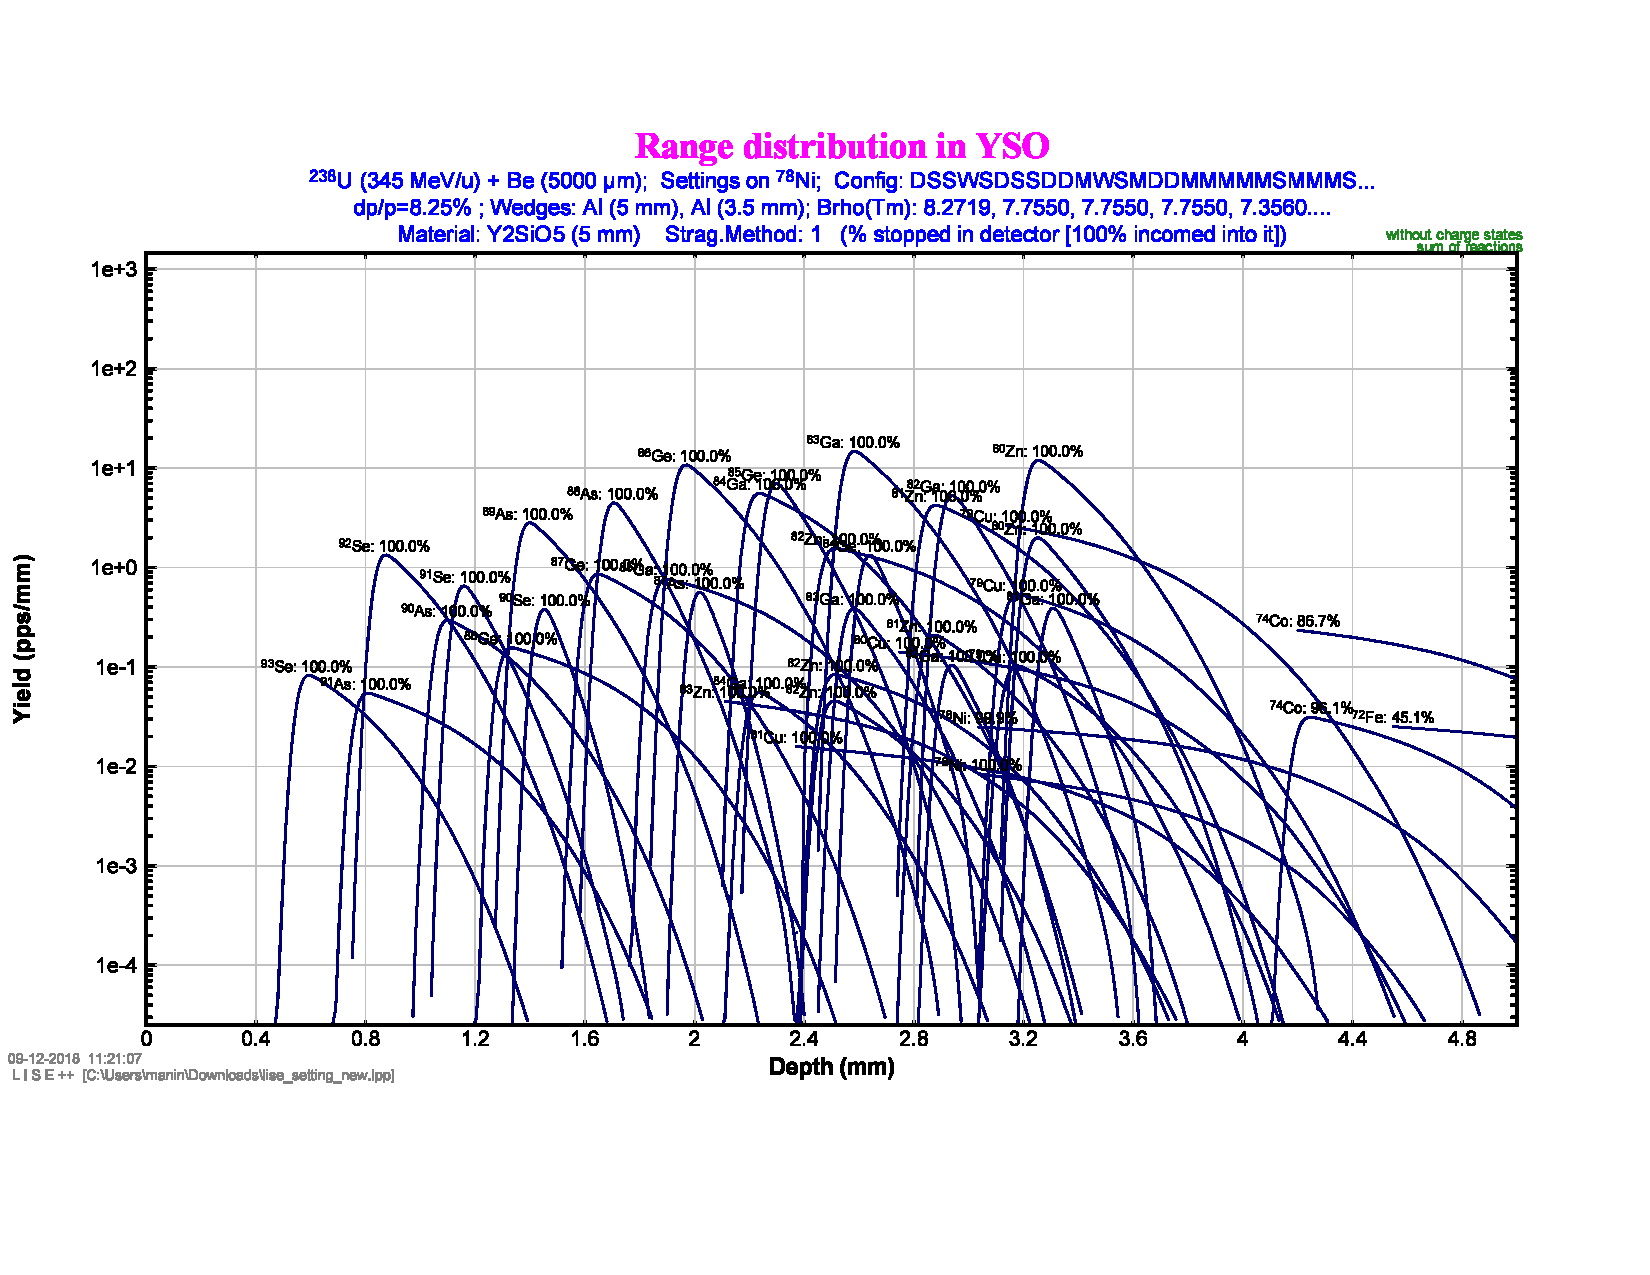
\includegraphics[height=16cm, width=17cm]{figures/yso_lise_snapshot-rotated.pdf}
	\caption[Range distribution of various ions in YSO]{Range distribution of various ions in YSO. The configuration for the calculations is reminiscent of the setup available at RIBF, RIKEN. The heaviest ions are implanted shallower with full absorption, lighter ions have relatively deeper implantation, requiring proper energy-degraders for total stoppage in YSO. }
	\label{fig:ionrangeyso}
\end{figure}

Electrons generated followed by the $\beta^{-}$-decay of these radioactive ions can have energy as low as a few keV or as high as a few MeV. Information about the range of electrons of various energy is also vital from the ion-$\beta$ correlation perspective. It is helpful in designing and optimizing the position gates around implant positions. These range estimates were produced using on internet program \textbf{ESTAR} \citep{estar}. Details about chemical composition and density are the input parameters to the program. The program calculates  stopping power, density effect parameters, range, and radiation yield tables for electrons in various materials.

\begin{figure}[h!]
	\centering
	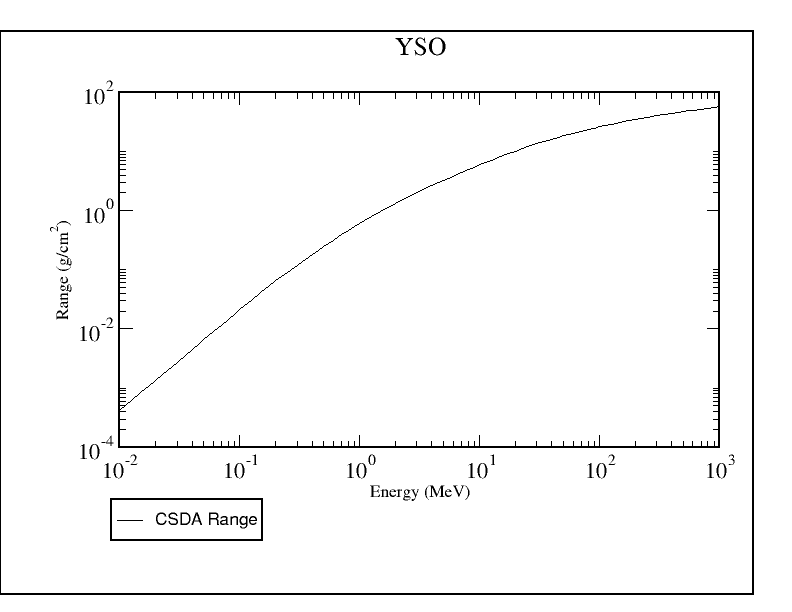
\includegraphics[width=10cm,height=8cm]{figures/yso_electrons_range.png}
	\caption[Continuous slowing down approximation range (CSDA)]{Continuous slowing down approximation range (CSDA) of electrons in YSO computed using ESTAR.}
	\label{fig:electron_range_yso}
\end{figure}
